
%%%%%%%%%%%%%%%%%%%%%%%%%%%%%%%%%%%%%%%%%%%%%%%%%%%%%%%%
%
% Copyright (c) 2003-2010 by University of Queensland
% Earth Systems Science Computational Center (ESSCC)
% http://www.uq.edu.au/esscc
%
% Primary Business: Queensland, Australia
% Licensed under the Open Software License version 3.0
% http://www.opensource.org/licenses/osl-3.0.php
%
%%%%%%%%%%%%%%%%%%%%%%%%%%%%%%%%%%%%%%%%%%%%%%%%%%%%%%%%


\section{The Diffusion Problem}
\label{DIFFUSION CHAP}

\begin{figure}
\centerline{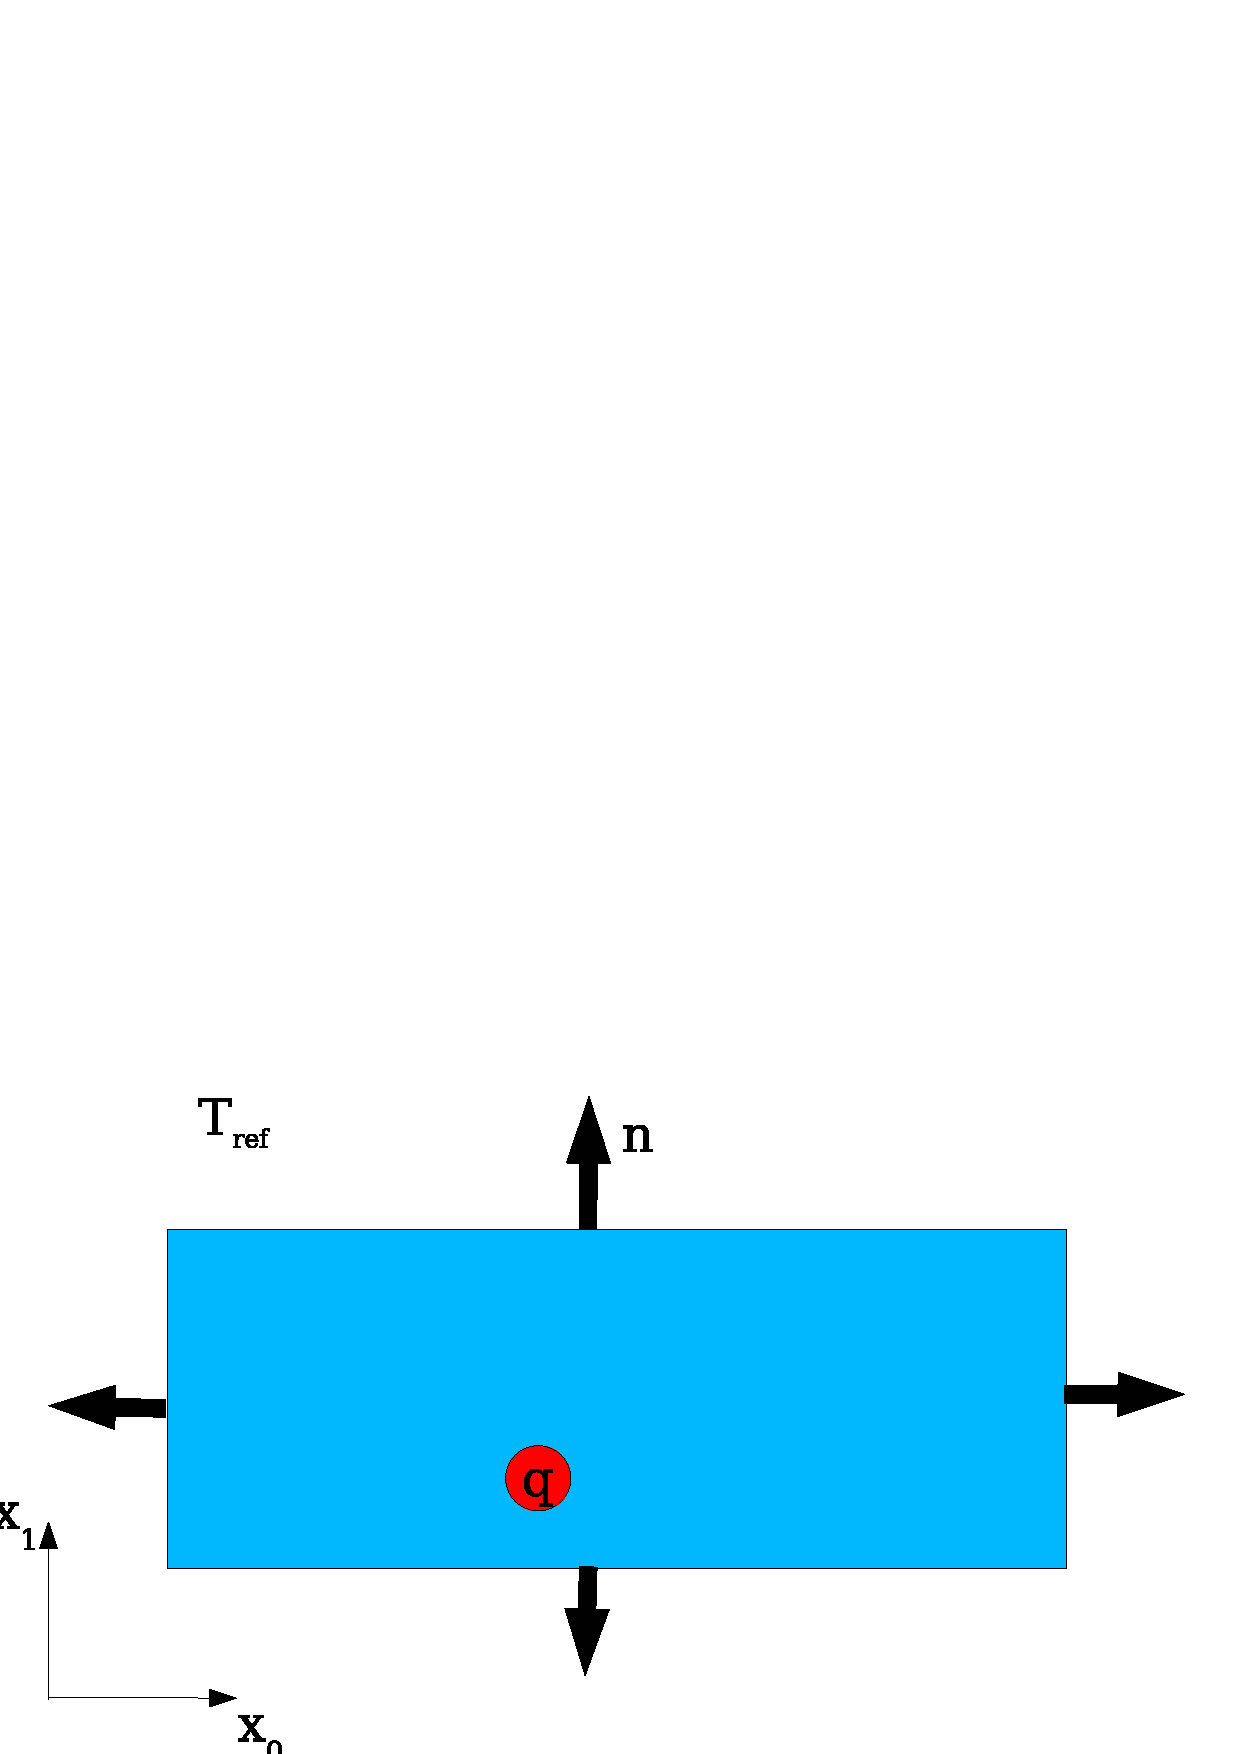
\includegraphics[width=\figwidth]{DiffusionDomain}}
\caption{Temperature Diffusion Problem with Circular Heat Source}
\label{DIFFUSION FIG 1}
\end{figure}

\subsection{\label{DIFFUSION OUT SEC}Outline}
In this chapter we will discuss how to solve a time-dependent temperature
diffusion\index{diffusion equation} PDE for a given block of material.
Within the block there is a heat source which drives the temperature diffusion.
On the surface, energy can radiate into the surrounding environment.
\fig{DIFFUSION FIG 1} shows the configuration.

In the next \Sec{DIFFUSION TEMP SEC} we will present the relevant model.
A time integration scheme is introduced to calculate the temperature at given time nodes $t^{(n)}$.
We will see that at each time step a Helmholtz equation\index{Helmholtz equation} must be solved. 
The implementation of a Helmholtz equation solver will be discussed in \Sec{DIFFUSION HELM SEC}. 
In Section~\ref{DIFFUSION TRANS SEC} this solver is used to build a solver for
the temperature diffusion problem.

\subsection{\label{DIFFUSION TEMP SEC}Temperature Diffusion}
The unknown temperature $T$ is a function of its location in the domain and time $t>0$.
The governing equation in the interior of the domain is given by
\begin{equation}
\rho c_p T_{,t} - (\kappa T_{,i})_{,i} = q_H
\label{DIFFUSION TEMP EQ 1}
\end{equation}
where $\rho c_p$ and $\kappa$ are given material constants.
In case of a composite material the parameters depend on their location in the domain.
$q_H$ is a heat source (or sink) within the domain.
We are using the Einstein summation convention\index{summation convention} as introduced in \Chap{FirstSteps}.
In our case we assume $q_H$ to be equal to a constant heat
production rate $q^{c}$ on a circle or sphere with center $x^c$ and radius $r$, and $0$ elsewhere:
\begin{equation}
q_H(x,t)=\left\{ 
\begin{array}{l l}
    q^c  & \quad\text{if $\|x-x^c\| \le r$}\\
    0    & \quad\text{else}\\
\end{array} \right.
\label{DIFFUSION TEMP EQ 1b}
\end{equation}
for all $x$ in the domain and time $t>0$.

On the surface of the domain we specify a radiation condition which prescribes
the normal component of the flux $\kappa T_{,i}$ to be proportional
to the difference of the current temperature to the surrounding temperature $T_{ref}$:
\begin{equation}
 \kappa T_{,i} n_i = \eta (T_{ref}-T) 
\label{DIFFUSION TEMP EQ 2}
\end{equation}
$\eta$ is a given material coefficient depending on the material of the block and the surrounding medium.
$n_i$ is the $i$-th component of the outer normal field\index{outer normal field} at the surface of the domain. 

To solve the time-dependent \eqn{DIFFUSION TEMP EQ 1} the initial temperature at time $t=0$ has to be given.
Here we assume that the initial temperature is the surrounding temperature:
\begin{equation}
T(x,0)=T_{ref} 
\label{DIFFUSION TEMP EQ 4}
\end{equation}
for all $x$ in the domain. Note that the initial conditions satisfy the
boundary condition defined by \eqn{DIFFUSION TEMP EQ 2}. 

The temperature is calculated at discrete time nodes $t^{(n)}$ where 
$t^{(0)}=0$ and $t^{(n)}=t^{(n-1)}+h$, where $h>0$ is the step size which is assumed to be constant.
In the following, the upper index ${(n)}$ refers to a value at time $t^{(n)}$.
The simplest and most robust scheme to approximate the time derivative of the
temperature is the backward Euler\index{backward Euler} scheme.
The backward Euler scheme is based on the Taylor expansion of $T$ at time $t^{(n)}$:
\begin{equation}
T^{(n)}\approx T^{(n-1)}+T_{,t}^{(n)}(t^{(n)}-t^{(n-1)})
=T^{(n-1)} + h \cdot T_{,t}^{(n)}
\label{DIFFUSION TEMP EQ 6}
\end{equation}
This is inserted into \eqn{DIFFUSION TEMP EQ 1}. By separating the terms at
$t^{(n)}$ and $t^{(n-1)}$ one gets for $n=1,2,3\ldots$
\begin{equation}
\frac{\rho c_p}{h} T^{(n)} - (\kappa T^{(n)}_{,i})_{,i} = q_H +  \frac{\rho c_p}{h} T^{(n-1)}
\label{DIFFUSION TEMP EQ 7}
\end{equation}
where $T^{(0)}=T_{ref}$ is taken form the initial condition given by \eqn{DIFFUSION TEMP EQ 4}.
Together with the natural boundary condition 
\begin{equation}
 \kappa T_{,i}^{(n)} n_i = \eta (T_{ref}-T^{(n)}) 
\label{DIFFUSION TEMP EQ 2222}
\end{equation}
taken from \eqn{DIFFUSION TEMP EQ 2} this forms a boundary value problem that
has to be solved for each time step. 
As a first step to implement a solver for the temperature diffusion problem we
will implement a solver for the boundary value problem that has to be solved
at each time step.

\subsection{\label{DIFFUSION HELM SEC}Helmholtz Problem}
The partial differential equation to be solved for $T^{(n)}$ has the form 
\begin{equation}
\omega T^{(n)} - (\kappa T^{(n)}_{,i})_{,i} = f
\label{DIFFUSION HELM EQ 1}
\end{equation}
and we set
\begin{equation}
\omega=\frac{\rho c_p}{h} \mbox{ and } f=q_H +\frac{\rho c_p}{h}T^{(n-1)} \;.
\label{DIFFUSION HELM EQ 1b}
\end{equation}
With $g=\eta T_{ref}$ the radiation condition defined by \eqn{DIFFUSION TEMP EQ 2222} takes the form 
\begin{equation}
    \kappa T^{(n)}_{,i} n_{i} = g - \eta T^{(n)}\text{ on $\Gamma$}
\label{DIFFUSION HELM EQ 2}
\end{equation}
The partial differential \eqn{DIFFUSION HELM EQ 1} together with boundary
conditions of \eqn{DIFFUSION HELM EQ 2} is called the Helmholtz equation\index{Helmholtz equation}.

We want to use the \LinearPDE class provided by \escript to define and solve a
general linear, steady, second order PDE such as the Helmholtz equation.
For a single PDE the \LinearPDE class supports the following form:
\begin{equation}\label{LINEARPDE.SINGLE.1 TUTORIAL}
-(A_{jl} u_{,l})_{,j}+D u = Y
\end{equation}
where we show only the coefficients relevant for the problem discussed here.
For the general form of a single PDE see \eqn{LINEARPDE.SINGLE.1}.
The coefficients $A$ and $Y$ have to be specified through \Data objects in
the \Function on the PDE or objects that can be converted into such \Data objects.
$A$ is a \RankTwo and $D$ and $Y$ are scalar.
The following natural boundary conditions\index{boundary condition!natural}
are considered on $\Gamma$:
\begin{equation}\label{LINEARPDE.SINGLE.2 TUTORIAL}
n_{j}A_{jl} u_{,l}+d u= y  \;.
\end{equation}
Notice that the coefficient $A$ is the same like in the PDE~\eqn{LINEARPDE.SINGLE.1 TUTORIAL}.
The coefficients $d$ and $y$ are each a \Scalar in the \FunctionOnBoundary.
Constraints\index{constraint} for the solution prescribe the value of the
solution at certain locations in the domain. They have the form
\begin{equation}\label{LINEARPDE.SINGLE.3 TUTORIAL}
u=r \mbox{ where } q>0
\end{equation}
$r$ and $q$ are each \Scalar where $q$ is the characteristic function\index{characteristic function} defining where the constraint is applied.
The constraints defined by \eqn{LINEARPDE.SINGLE.3 TUTORIAL} override any
other condition set by \eqn{LINEARPDE.SINGLE.1 TUTORIAL} or \eqn{LINEARPDE.SINGLE.2 TUTORIAL}.
The \Poisson class of the \linearPDEs module, which we have already used in
\Chap{FirstSteps}, is in fact a subclass of the more general \LinearPDE class.
The \linearPDEs module provides a \Helmholtz class but we will make direct use
of the general \LinearPDE class.

By inspecting the Helmholtz equation\index{Helmholtz equation}
(\ref{DIFFUSION HELM EQ 1}) and boundary condition (\ref{DIFFUSION HELM EQ 2}),
and substituting $u$ for $T^{(n)}$, we can easily assign values to the
coefficients in the general PDE of the \LinearPDE class:
\begin{equation}\label{DIFFUSION HELM EQ 3}
\begin{array}{llllll}
A_{ij}=\kappa \delta_{ij} & D=\omega & Y=f \\
d=\eta & y= g &  \\
\end{array}
\end{equation}
$\delta_{ij}$ is the Kronecker symbol\index{Kronecker symbol} defined
by $\delta_{ij}=1$ for $i=j$ and $0$ otherwise.
Undefined coefficients are assumed to be not present.\footnote{There is a
difference in \escript for a coefficient to be not present and set to zero.
Since in the former case the coefficient is not processed, it is more efficient
to leave it undefined instead of assigning zero to it.}
In this diffusion example we do not need to define a characteristic function
$q$ because the boundary conditions we consider in \eqn{DIFFUSION HELM EQ 2}
are just the natural boundary conditions which are already defined in the
\LinearPDE class (shown in \eqn{LINEARPDE.SINGLE.2 TUTORIAL}).

The Helmholtz equation can be set up the following way\footnote{Note that this
is not a complete code. The full source code can be found in ``helmholtz.py''.}:
\begin{python}
  mypde=LinearPDE(mydomain)
  mypde.setValue(A=kappa*kronecker(mydomain),D=omega,Y=f,d=eta,y=g)
  u=mypde.getSolution()
\end{python}
where we assume that \code{mydomain} is a \Domain object and 
\code{kappa}, \code{omega}, \code{eta}, and \code{g} are given scalar values
typically \code{float} or \Data objects. The \method{setValue} method
assigns values to the coefficients of the general PDE.
The \method{getSolution} method solves the PDE and returns the solution
\code{u} of the PDE. \function{kronecker} is an \escript function returning
the Kronecker symbol.

The coefficients can set by several calls to \method{setValue} where the order
can be chosen arbitrarily. 
If a value is assigned to a coefficient several times, the last assigned value
is used when the solution is calculated:
\begin{python}
  mypde = LinearPDE(mydomain)
  mypde.setValue(A=kappa*kronecker(mydomain), d=eta)
  mypde.setValue(D=omega, Y=f, y=g)
  mypde.setValue(d=2*eta) # overwrites d=eta
  u=mypde.getSolution()
\end{python}
In some cases the solver of the PDE can make use of the fact that the PDE is
symmetric\index{symmetric PDE}. A PDE is called symmetric if
\begin{equation}\label{LINEARPDE.SINGLE.4  TUTORIAL}
A_{jl}=A_{lj}\;.
\end{equation}
Note that $D$ and $d$ may have any value and the right hand sides $Y$, $y$ as
well as the constraints are not relevant. The Helmholtz problem is symmetric.
The \LinearPDE class provides the method \method{checkSymmetry} to check if
the given PDE is symmetric.
\begin{python}
  mypde = LinearPDE(mydomain)
  mypde.setValue(A=kappa*kronecker(mydomain), d=eta)
  print mypde.checkSymmetry() # returns True
  mypde.setValue(B=kronecker(mydomain)[0])
  print mypde.checkSymmetry() # returns False
  mypde.setValue(C=kronecker(mydomain)[0])
  print mypde.checkSymmetry() # returns True
\end{python}
Unfortunately, calling \method{checkSymmetry} is very expensive and is only
recommended for testing and debugging purposes.
The \method{setSymmetryOn} method is used to declare a PDE symmetric:
\begin{python}
  mypde = LinearPDE(mydomain)
  mypde.setValue(A=kappa*kronecker(mydomain))
  mypde.setSymmetryOn()
\end{python}
Now we want to see how we actually solve the Helmholtz equation on a
rectangular domain of length $l_{0}=5$ and height $l_{1}=1$.
We choose a simple test solution such that we can verify the returned solution
against the exact answer. Actually, we take $T=x_{0}$ (here
$q_H = 0$) and then calculate the right hand side terms $f$ and $g$
such that the test solution becomes the solution of the problem.
If we assume $\kappa$ as being constant, an easy calculation shows that we
have to choose $f=\omega \cdot x_{0}$.
On the boundary we get $\kappa n_{i} u_{,i}=\kappa n_{0}$.
Thus we have to set $g=\kappa n_{0}+\eta x_{0}$.
The following script \file{helmholtz.py}\index{scripts!\file{helmholtz.py}}
which is available in the \ExampleDirectory implements this test problem using
the \finley PDE solver:
\begin{python}
  from esys.escript import *
  from esys.escript.linearPDEs import LinearPDE
  from esys.finley import Rectangle
  from esys.weipa import saveVTK
  # set some parameters
  kappa=1.
  omega=0.1
  eta=10.
  # generate domain
  mydomain = Rectangle(l0=5., l1=1., n0=50, n1=10)
  # open PDE and set coefficients
  mypde=LinearPDE(mydomain)
  mypde.setSymmetryOn()
  n=mydomain.getNormal()
  x=mydomain.getX()
  mypde.setValue(A=kappa*kronecker(mydomain), D=omega,Y=omega*x[0], \
                 d=eta, y=kappa*n[0]+eta*x[0])
  # calculate error of the PDE solution
  u=mypde.getSolution()
  print("error is ",Lsup(u-x[0]))
  saveVTK("x0.vtu", sol=u)
\end{python}
To visualize the solution `x0.vtu' you can use the command
\begin{verbatim}
mayavi -d x0.vtu -m SurfaceMap
\end{verbatim}
and it is easy to see that the solution $T=x_{0}$ is calculated.
 
The script is similar to the script \file{poisson.py} discussed in \Chap{FirstSteps}.
\code{mydomain.getNormal()} returns the outer normal field on the surface of the domain.
The function \function{Lsup} is imported by the \code{from esys.escript import *}
statement and returns the maximum absolute value of its argument.
The error shown by the print statement should be in the order of $10^{-7}$.
As piecewise bi-linear interpolation is used by \finley to approximate the
solution, and our solution is a linear function of the spatial coordinates,
one might expect that the error would be zero or in the order of machine
precision (typically $\approx 10^{-15}$).
However most PDE packages use an iterative solver which is terminated when a
given tolerance has been reached. The default tolerance is $10^{-8}$.
This value can be altered by using the \method{setTolerance} of the \LinearPDE class.

\subsection{The Transition Problem}
\label{DIFFUSION TRANS SEC}
Now we are ready to solve the original time-dependent problem. The main 
part of the script is the loop over time $t$ which takes the following form:
\begin{python}
  t=0
  T=Tref
  mypde=LinearPDE(mydomain)
  mypde.setValue(A=kappa*kronecker(mydomain), D=rhocp/h, d=eta, y=eta*Tref)
  while t<t_end:
        mypde.setValue(Y=q+rhocp/h*T)
        T=mypde.getSolution()
        t+=h
\end{python}
\var{kappa}, \var{rhocp}, \var{eta} and \var{Tref} are input parameters of the model.
\var{q} is the heat source in the domain and \var{h} is the time step size.
The variable \var{T} holds the current temperature.
It is used to calculate the right hand side coefficient \var{f} in the
Helmholtz \eqn{DIFFUSION HELM EQ 1}.
The statement \code{T=mypde.getSolution()} overwrites \var{T} with the
temperature of the new time step $\var{t}+\var{h}$.
To get this iterative process going we need to specify the initial temperature
distribution, which is equal to $T_{ref}$.
The \LinearPDE object \var{mypde} and the coefficients that do not change over
time are set up before the loop is entered.
In each time step only the coefficient $Y$ is reset as it depends on the
temperature of the previous time step.
This allows the PDE solver to reuse information from previous time steps as
much as possible.

The heat source $q_H$ which is defined in \eqn{DIFFUSION TEMP EQ 1b}
is \var{qc} in an area defined as a circle of radius \var{r} and center
\var{xc}, and zero outside this circle. \var{q0} is a fixed constant.
The following script defines $q_H$ as desired:
\begin{python}
  from esys.escript import length,whereNegative
  xc=[0.02, 0.002]
  r=0.001
  x=mydomain.getX()
  qH=q0*whereNegative(length(x-xc)-r)
\end{python}
\var{x} is a \Data object of the \escript module defining locations in the \Domain \var{mydomain}.
The \function{length()} function imported from the \escript module returns the 
Euclidean norm:
\begin{equation}\label{DIFFUSION HELM EQ 3aba}
\|y\|=\sqrt{
y_{i}
y_{i}
} = \function{esys.escript.length}(y)
\end{equation}
So \code{length(x-xc)} calculates the distances of the location \var{x} to the
center of the circle \var{xc} where the heat source is acting.
Note that the coordinates of \var{xc} are defined as a list of floating point numbers.
It is automatically converted into a \Data class object before being
subtracted from \var{x}.
The function \function{whereNegative} applied to \code{length(x-xc)-r} returns
a \Data object which is equal to one where the object is negative (inside the
circle) and zero elsewhere.
After multiplication with \var{qc} we get a function with the desired property
of having value \var{qc} inside the circle and zero elsewhere.

Now we can put the components together to create the script \file{diffusion.py}
which is available in the \ExampleDirectory\index{scripts!\file{diffusion.py}}:
\begin{python}
  from esys.escript import *
  from esys.escript.linearPDEs import LinearPDE
  from esys.finley import Rectangle
  from esys.weipa import saveVTK
  #... set some parameters ...
  xc=[0.02, 0.002]
  r=0.001
  qc=50.e6
  Tref=0.
  rhocp=2.6e6
  eta=75.
  kappa=240.
  tend=5.
  # ... time, time step size and counter ...
  t=0
  h=0.1
  i=0
  #... generate domain ...
  mydomain = Rectangle(l0=0.05, l1=0.01, n0=250, n1=50)
  #... open PDE ...
  mypde=LinearPDE(mydomain)
  mypde.setSymmetryOn()
  mypde.setValue(A=kappa*kronecker(mydomain), D=rhocp/h, d=eta, y=eta*Tref)
  # ... set heat source: ....
  x=mydomain.getX()
  qH=qc*whereNegative(length(x-xc)-r)
  # ... set initial temperature ....
  T=Tref
  # ... start iteration:
  while t<tend:
        i+=1
        t+=h
        print("time step:",t)
        mypde.setValue(Y=qH+rhocp/h*T)
        T=mypde.getSolution()
        saveVTK("T.%d.vtu"%i, temp=T)
\end{python}
The script will create the files \file{T.1.vtu}, \file{T.2.vtu}, $\ldots$,
\file{T.50.vtu} in the directory where the script has been started.
The files contain the temperature distributions at time steps $1, 2, i,
\ldots, 50$ in the \VTK file format.

\begin{figure}
\centerline{
\includegraphics[width=\figwidth]{DiffusionRes1}}
\centerline{
\includegraphics[width=\figwidth]{DiffusionRes16}}
\centerline{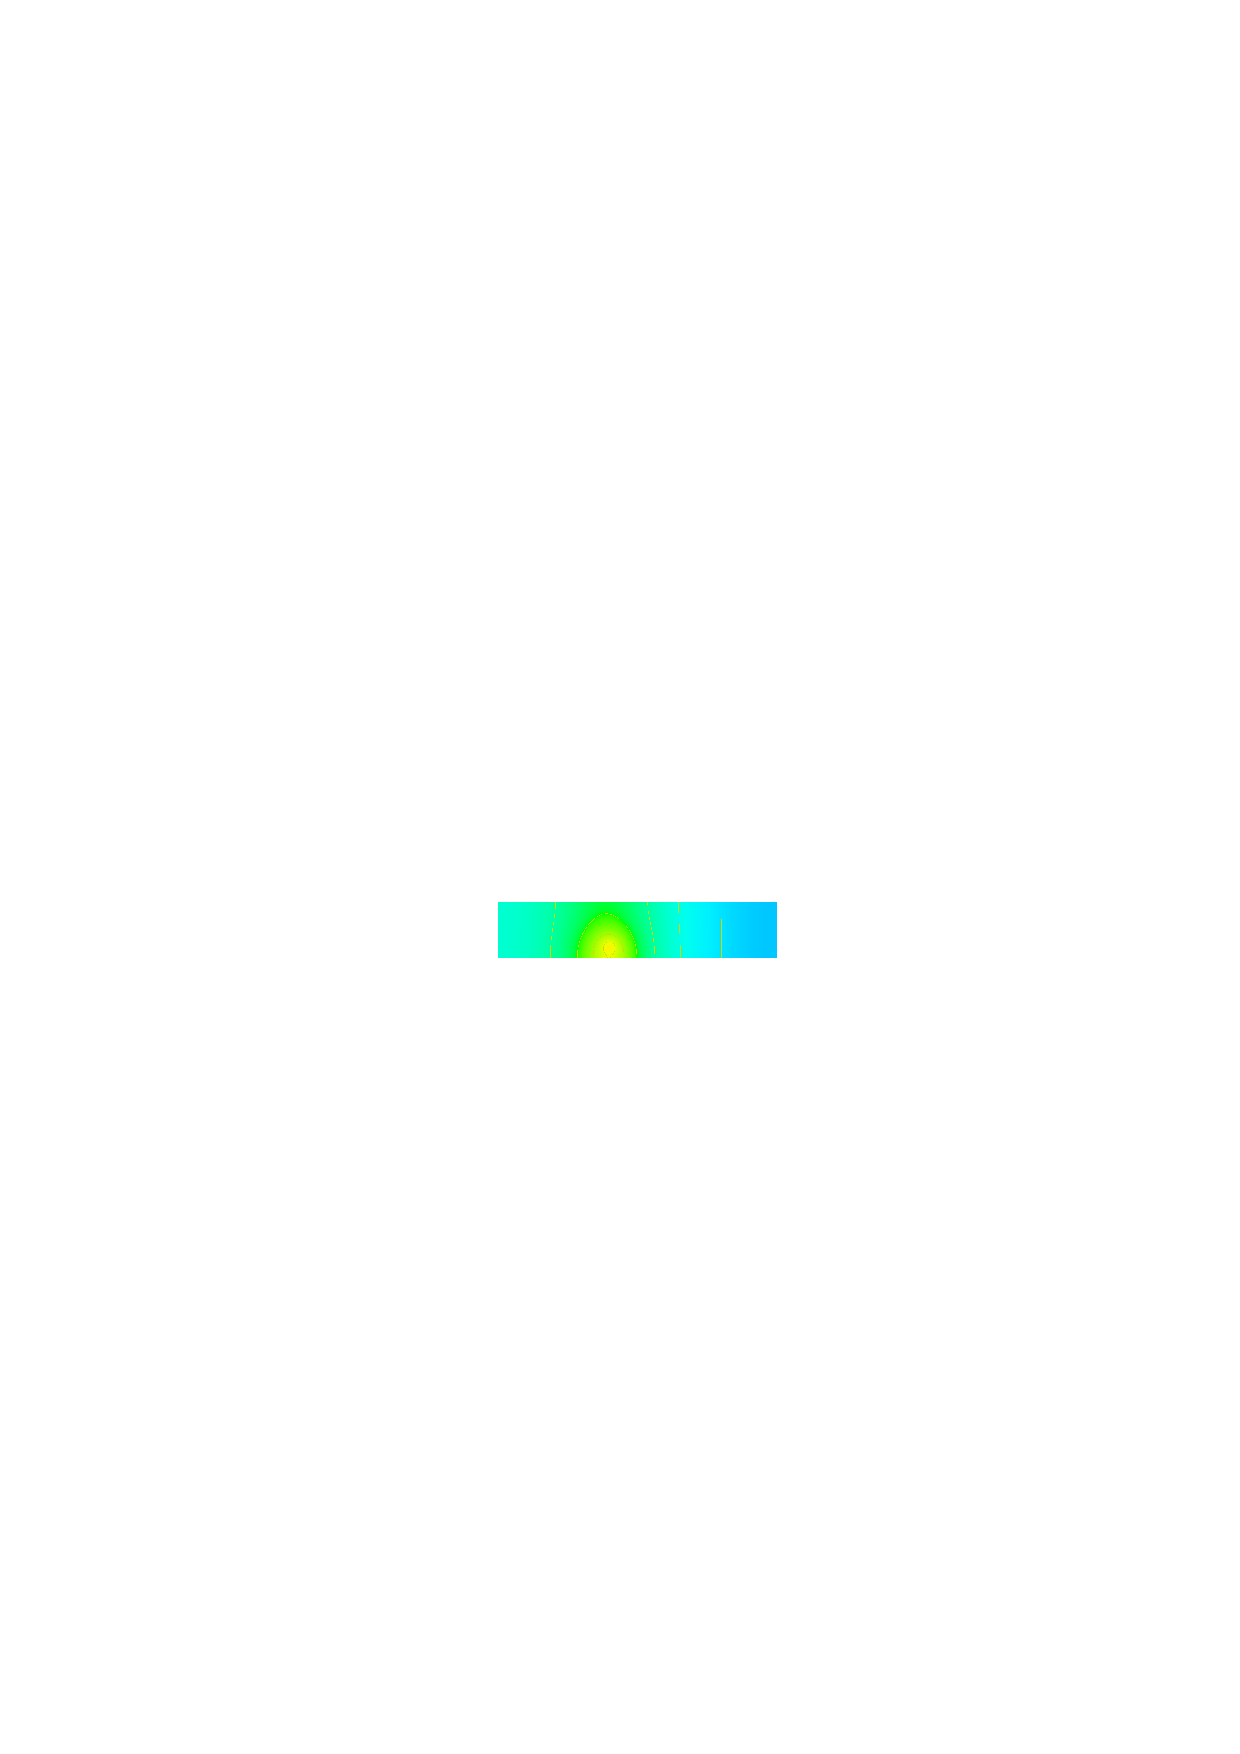
\includegraphics[width=\figwidth]{DiffusionRes32}}
\centerline{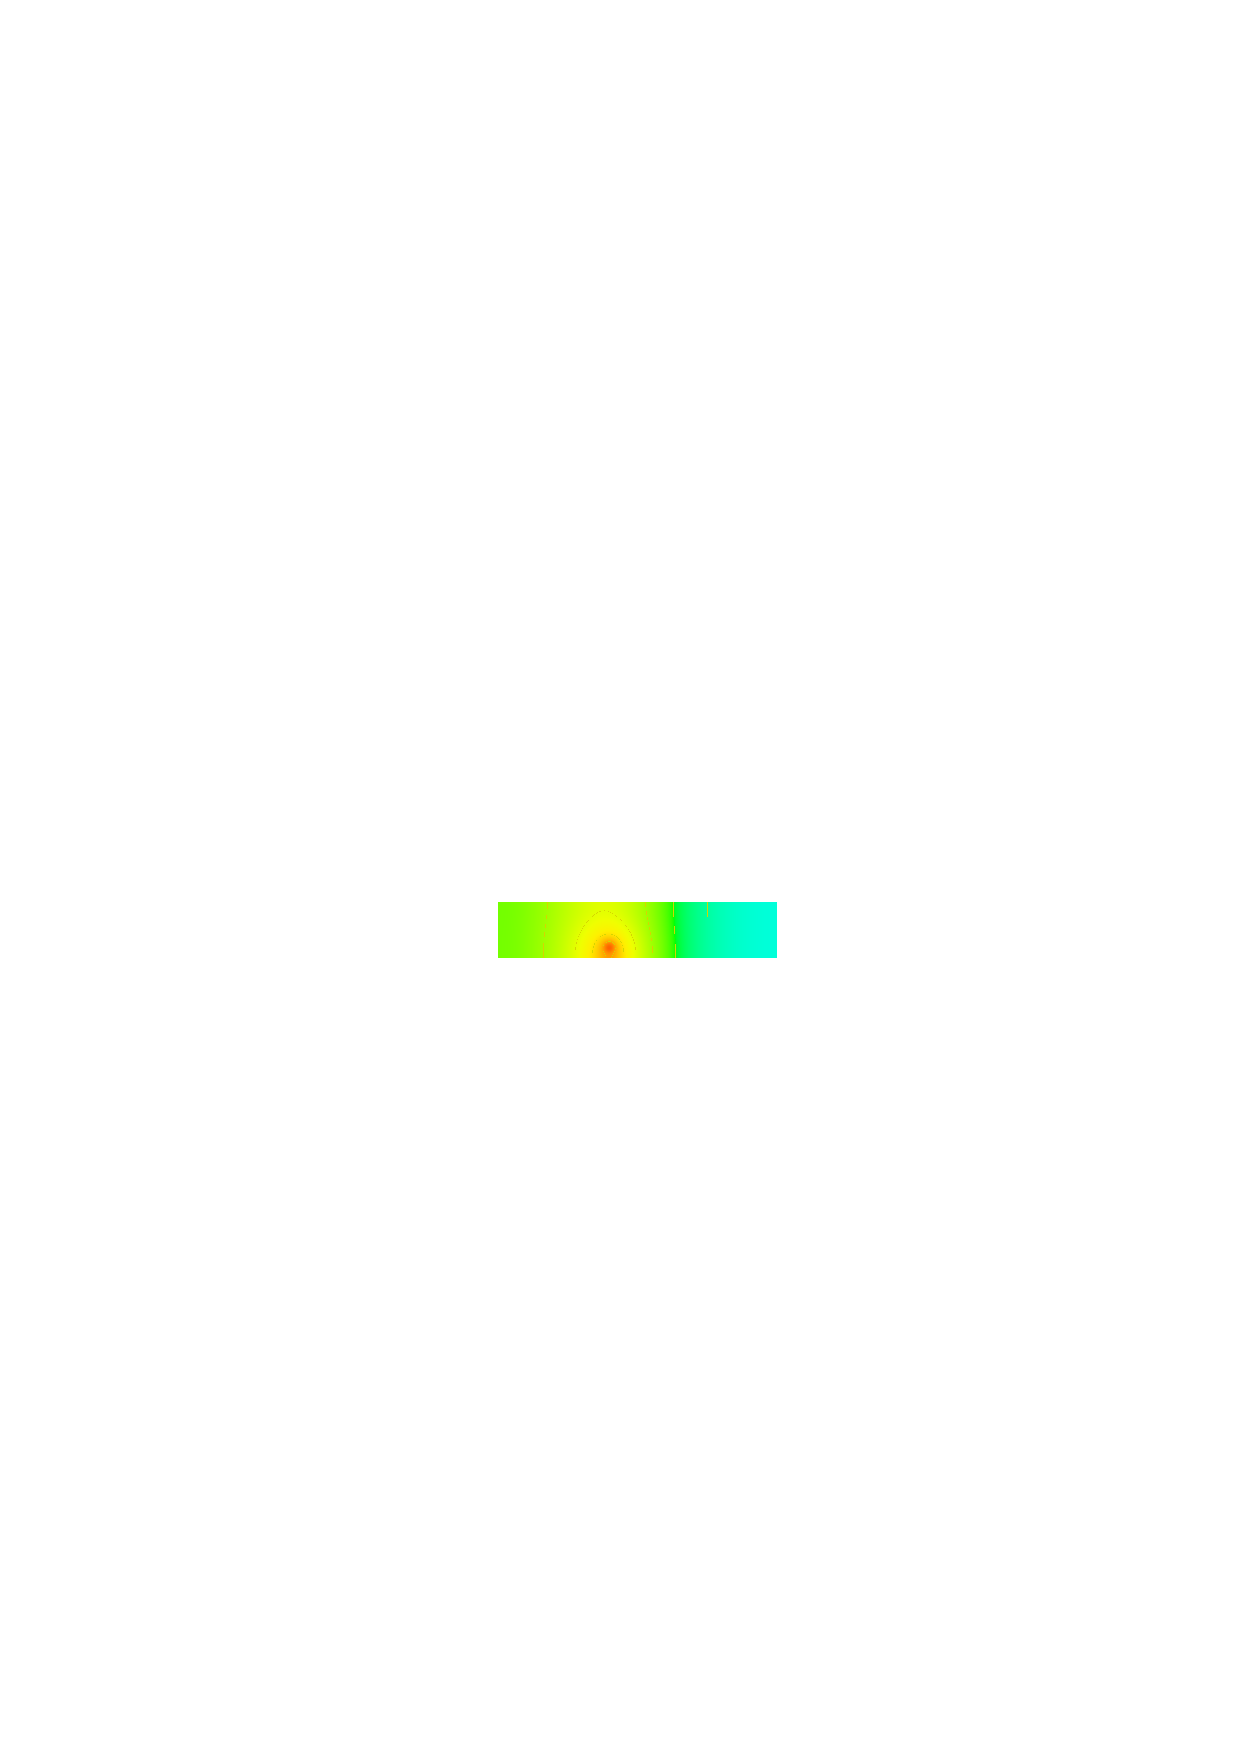
\includegraphics[width=\figwidth]{DiffusionRes48}}
\caption{Results of the Temperature Diffusion Problem for Time Steps 1, 16, 32 and 48}
\label{DIFFUSION FIG 2}
\end{figure}
\fig{DIFFUSION FIG 2} shows the result for some selected time steps.
An easy way to visualize the results is the command
\begin{verbatim}
mayavi -d T.1.vtu -m SurfaceMap
\end{verbatim}
Use the \emph{Configure Data} window in mayavi to move forward and backward in time.

